\section{题目一}
\subsection{实验目的}
安装配置UNIX V6++的运行环境。
\subsection{实验内容}
\begin{enumerate}
    \item 安装后端服务根证书;
    \item 登录实验平台;
    \item  运行远程桌面环境;
    \item 初始化代码仓库;
    \item 启动UNIX V6++运行环境。
\end{enumerate}
\subsection{实验过程}
安装完后端服务根证书后,登录网站http://vesper-system.pages.tongji.edu.cn/vesper-front/,然后如图\ref{changeCode}所示,修改密码。接着,如图
\ref{changeName}所示,修改主机名。之后,我在GitLab中创建了自己的代码分支。等待桌面环境启用后,如图\ref{genCode}所示,生成密钥,然后如图\ref{setCode}所示,将公钥上传至GitLab。
当我尝试下载实验工具包时,要求我输入用户名和密码,为此,为如图\ref{setToken}所示,申请了个人访问令牌用作密码。下载完成后,将工作目录设置为unix-v6pp-tongji,然后如图\ref{init},\ref{makeQemu},\ref{qemu}所示,依次执行init.sh和make qemu命令,
最终启动了UNIX V6++界面并如图\ref{helloWorld}所示,执行了echo命令。

\begin{figure}[!htbp]
    \centering
    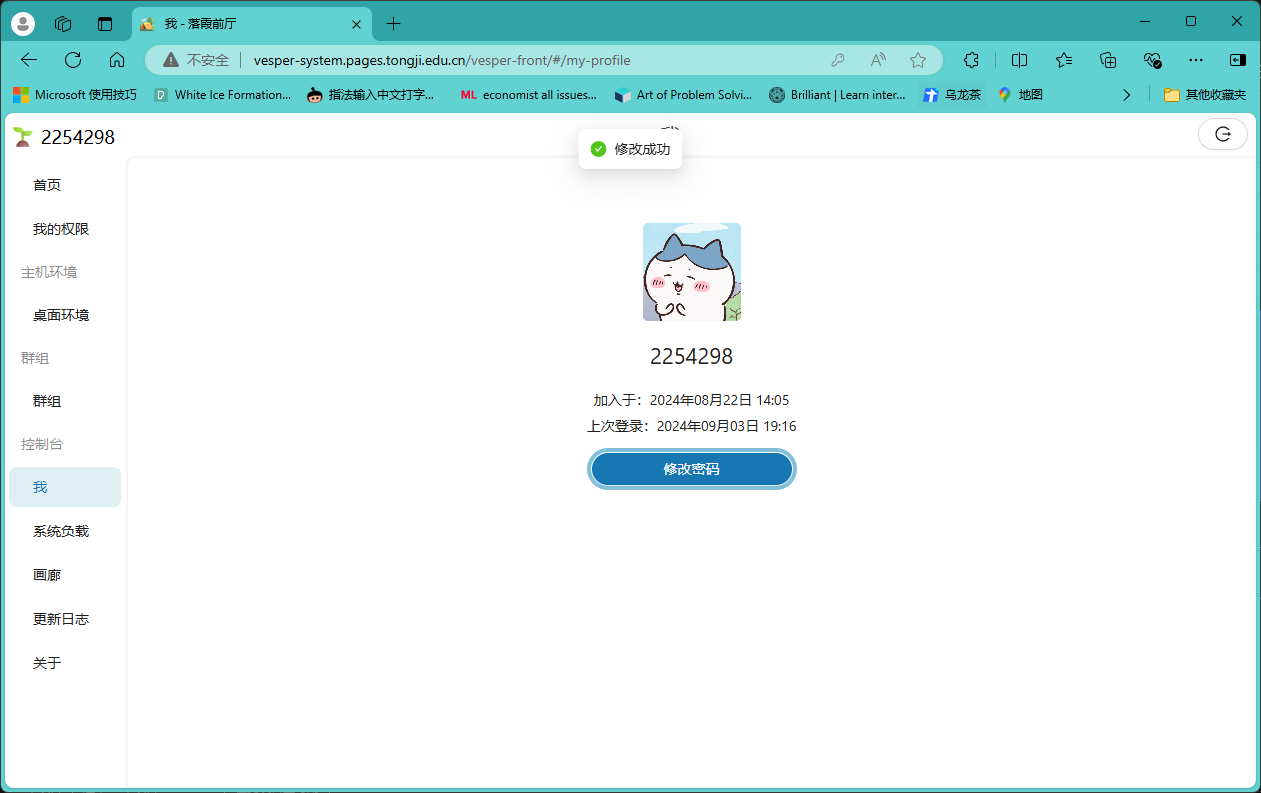
\includegraphics[scale=0.4]{fig/changeCode.png}
    \caption{修改密码}\label{changeCode}
\end{figure}
\begin{figure}[!htbp]
    \centering
    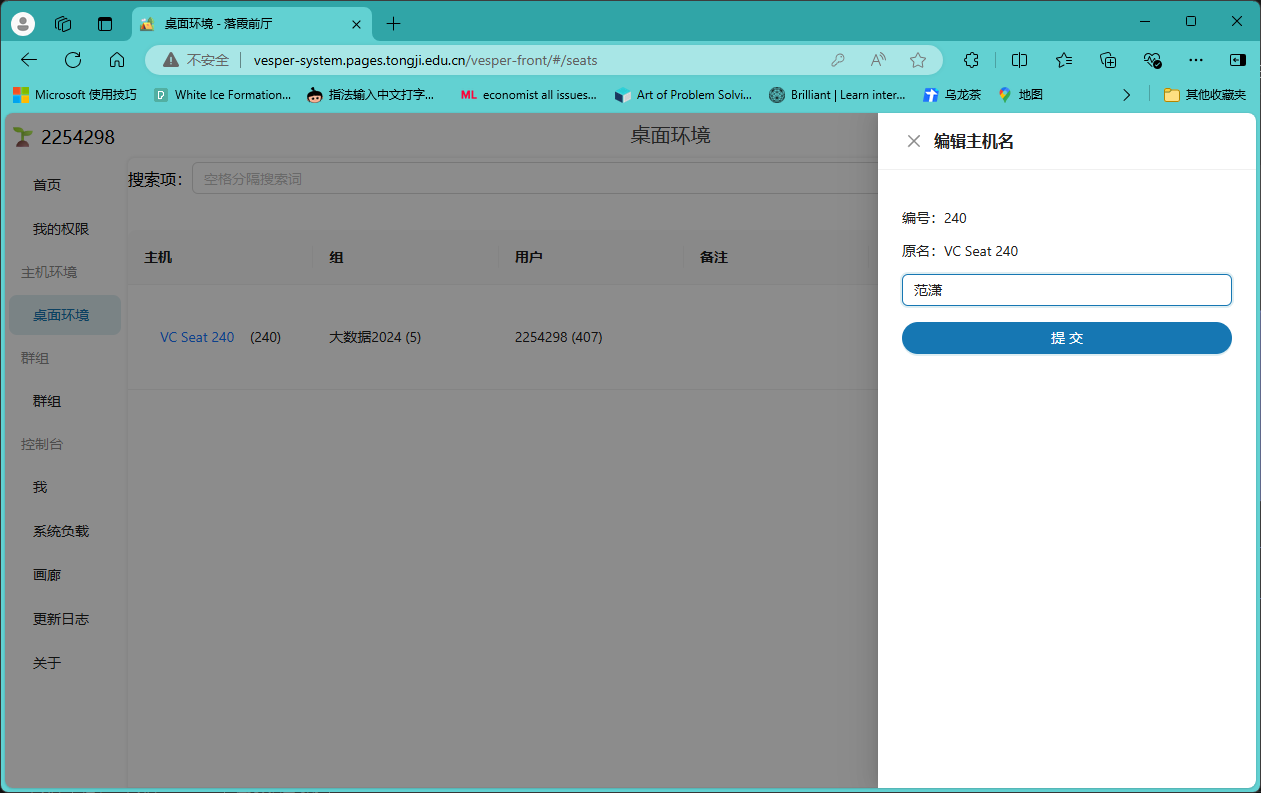
\includegraphics[scale=0.4]{fig/changeName.png}
    \caption{修改主机名}\label{changeName}
\end{figure}

\begin{figure}[!htbp]
    \centering
    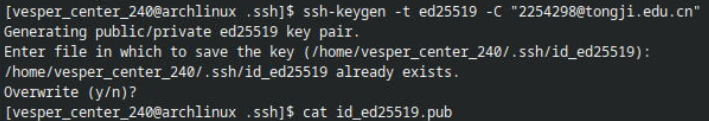
\includegraphics[scale=0.7]{fig/genCode.png}
    \caption{生成密钥}\label{genCode}
\end{figure}

\begin{figure}[!htbp]
    \centering
    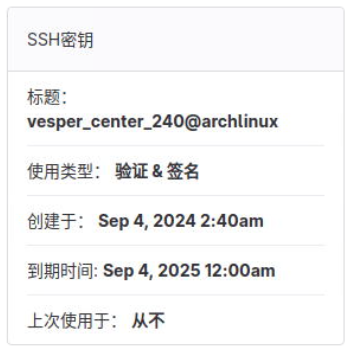
\includegraphics[scale=1]{fig/setCode.png}
    \caption{在GitLab中上传公钥}\label{setCode}
\end{figure}

\begin{figure}[!htbp]
    \centering
    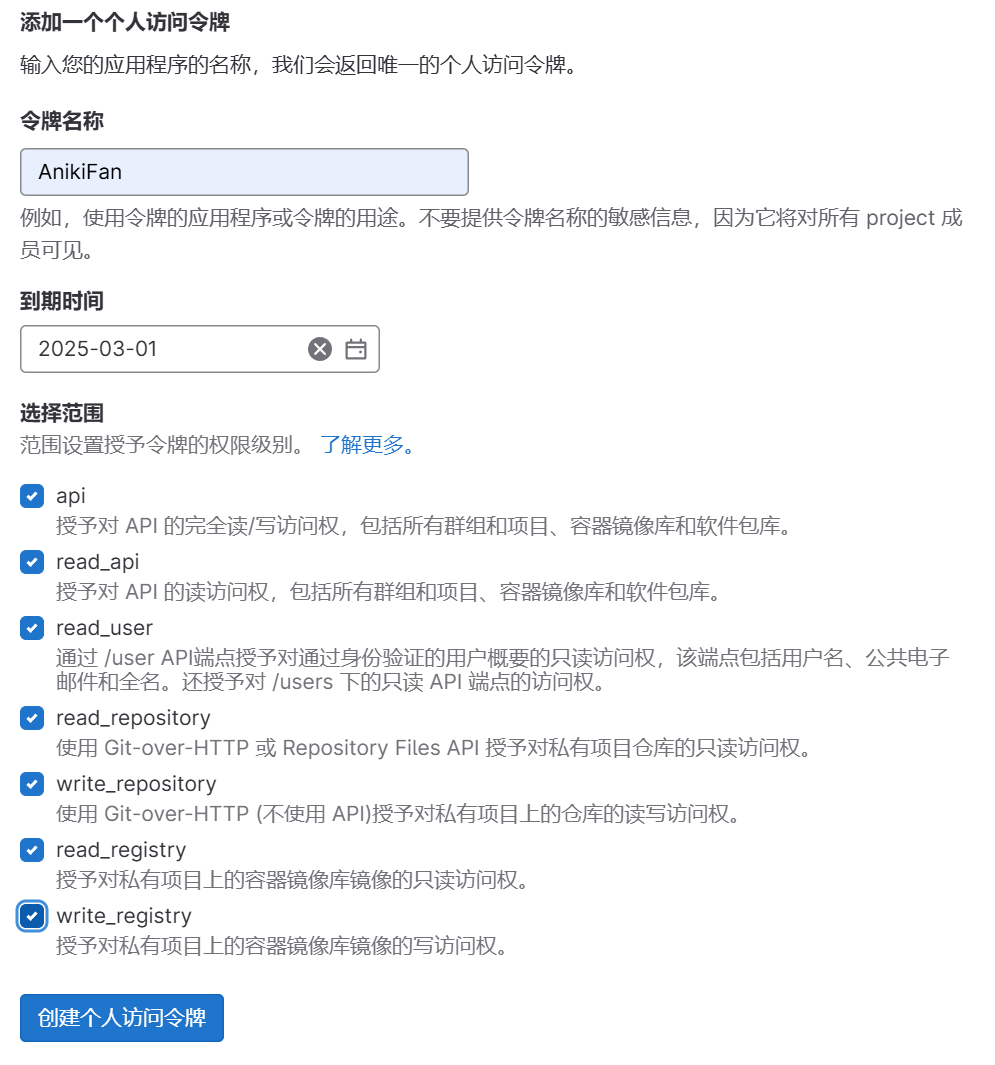
\includegraphics[scale=0.4]{fig/setToken.png}
    \caption{设置个人访问令牌}\label{setToken}
\end{figure}

\begin{figure}[!htbp]
    \centering
    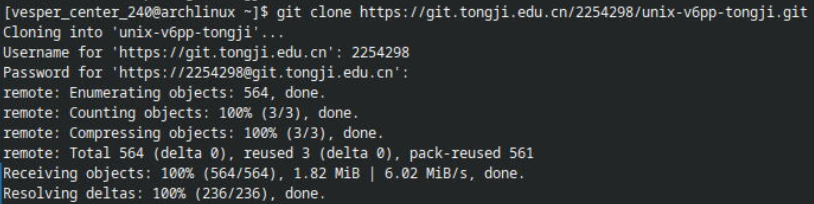
\includegraphics[scale=0.4]{fig/downloadTool.png}
    \caption{下载实验工具包}\label{downloadTool}
\end{figure}

\begin{figure}[!htbp]
    \centering
    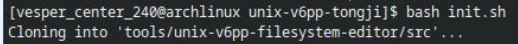
\includegraphics[scale=1]{fig/init.png}
    \caption{执行init.sh}\label{init}
\end{figure}

\begin{figure}[!htbp]
    \centering
    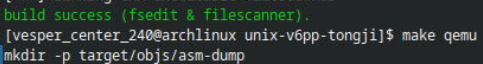
\includegraphics[scale=1]{fig/makeQemu.png}
    \caption{执行make qemu}\label{makeQemu}
\end{figure}

\begin{figure}[!htbp]
    \centering
    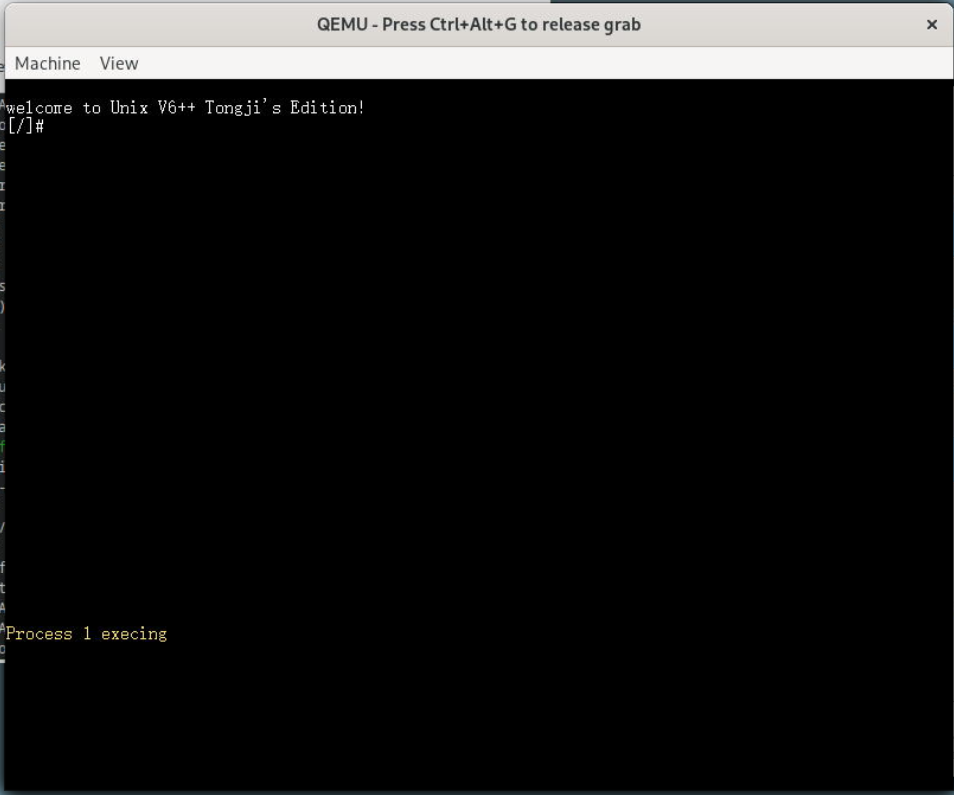
\includegraphics[scale=0.5]{fig/qemu.png}
    \caption{UNIX V6++界面}\label{qemu}
\end{figure}

\begin{figure}[!htbp]
    \centering
    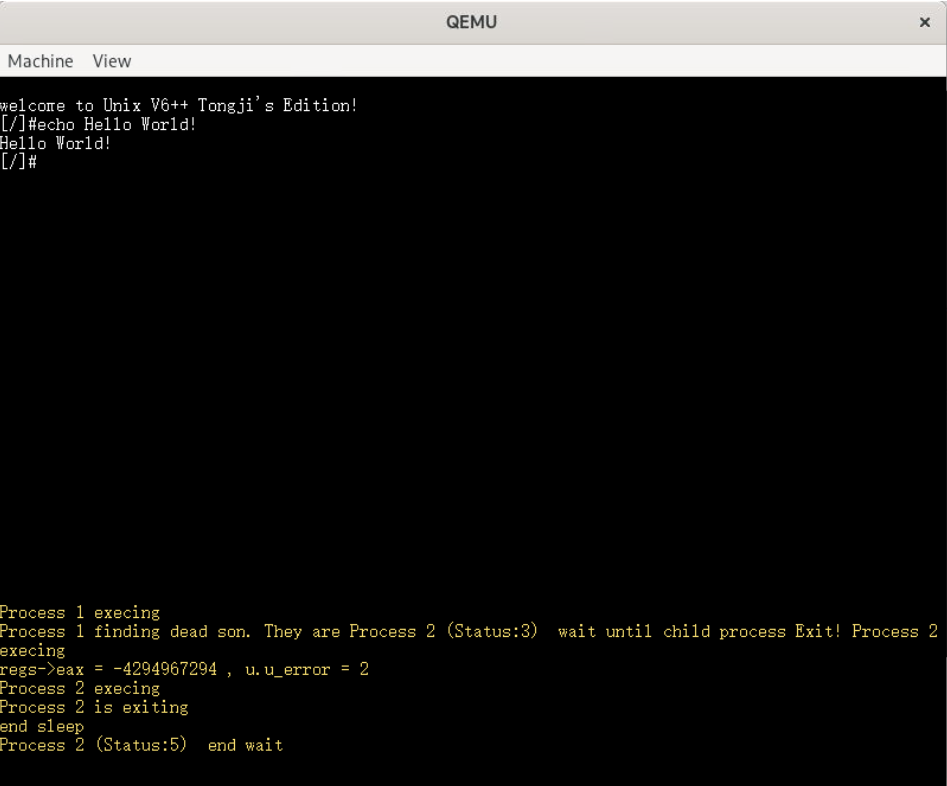
\includegraphics[scale=0.5]{fig/helloWorld.png}
    \caption{执行echo命令}\label{helloWorld}
\end{figure}
